% Appendices are set up same as chapter sections
\chapter{Appendix - Engineering Drawings and CAD Models}
\label{appendix:Appendix_eng}

\section{The Platform}

\begin{figure}
\centering
 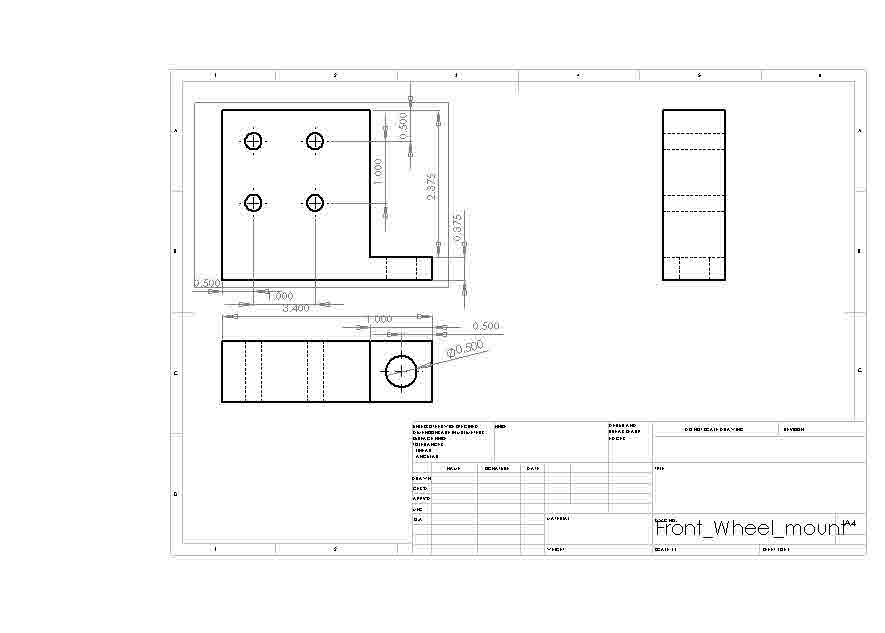
\includegraphics[width=0.8\textwidth]{images/Front_Wheel_mount}
\caption{The bracket mounted to the front of the platform for attaching the front casters}
\label{fig:front_bracket}
\end{figure}

\begin{figure}
\centering
 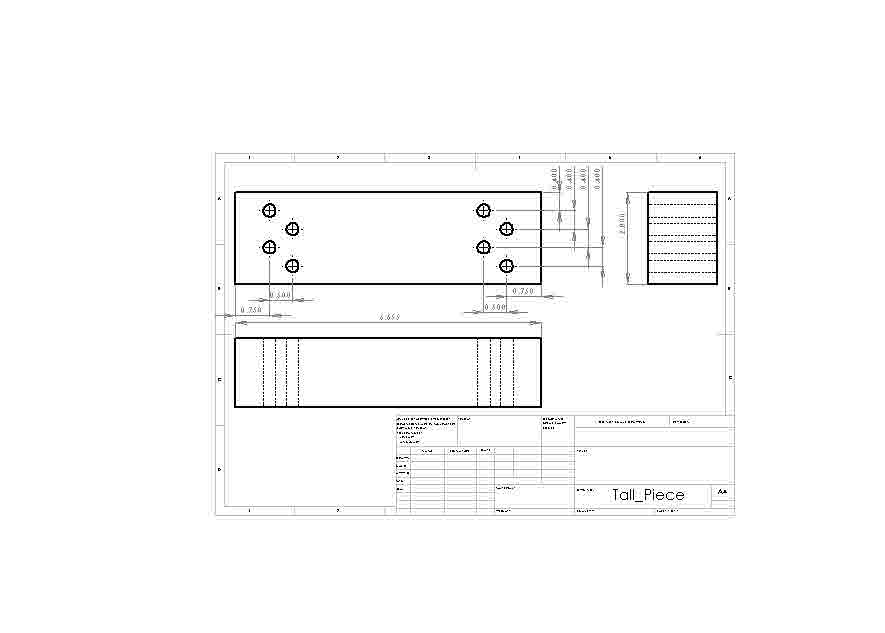
\includegraphics[width=0.8\textwidth]{images/Tall_Piece}
\caption{The piece bridging the bracket attached to the rear of the platform and the bracket attached to the jack}
\label{fig:tall_piece}
\end{figure}

\begin{figure}
\centering
 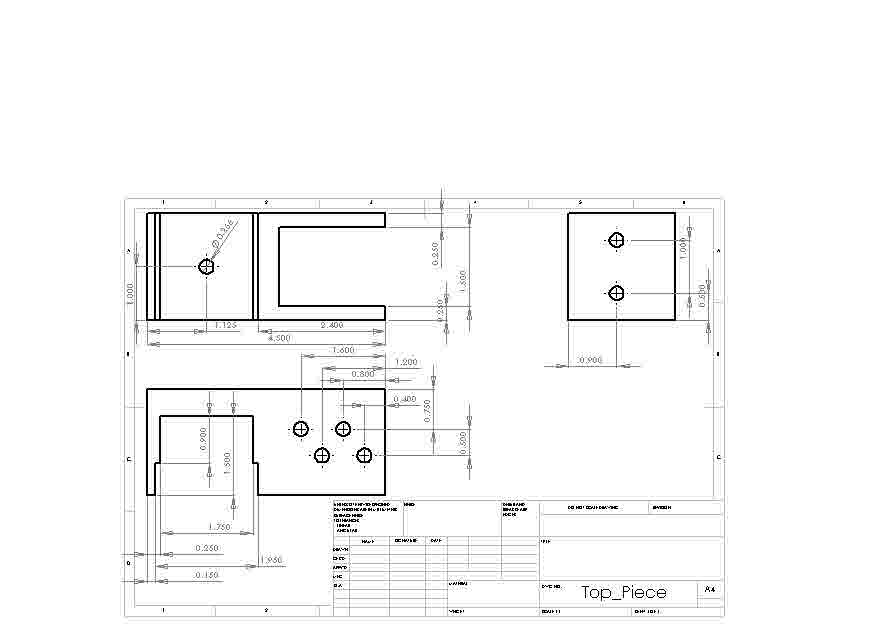
\includegraphics[width=0.8\textwidth]{images/Top_Piece}
\caption{The bracket for attaching to the electric jack}
\label{fig:top_piece}
\end{figure}

\begin{figure}
\centering
 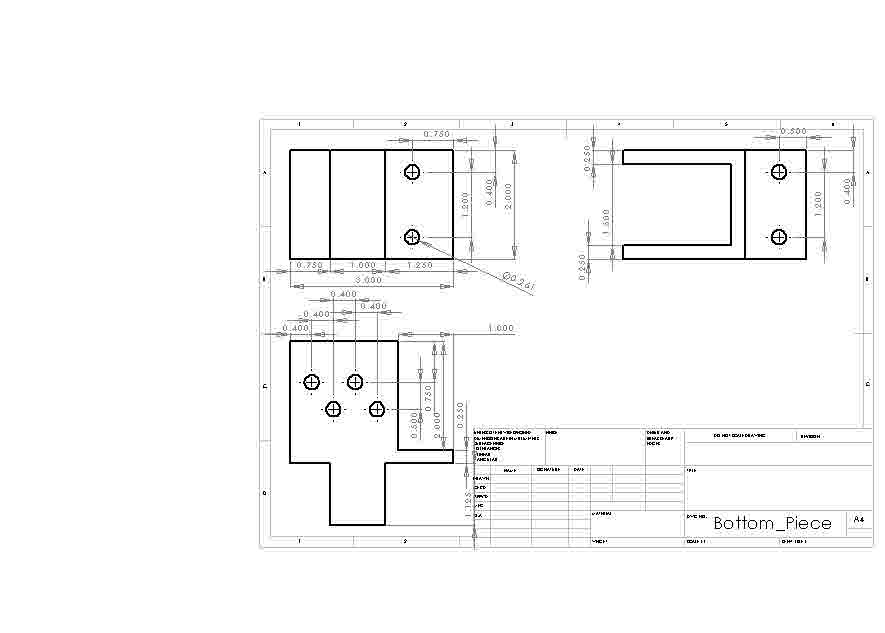
\includegraphics[width=0.8\textwidth]{images/Bottom_Piece}
\caption{The bracket for attaching to the rear of the platform}
\label{fig:bottom_piece}
\end{figure}

\newpage

\section{The Aisle Wheelchair}

\begin{figure}[h]
\centering
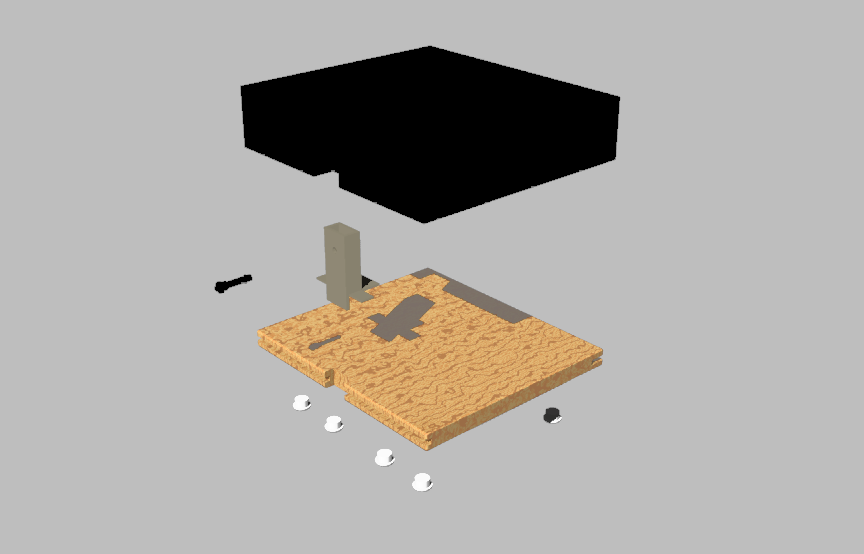
\includegraphics[width=7cm]{images/vistaex1.png}
\caption{Exploded view of the sliding base and cushion}
\label{fig:vistaex1}
\end{figure}

\begin{figure}[h]
\centering
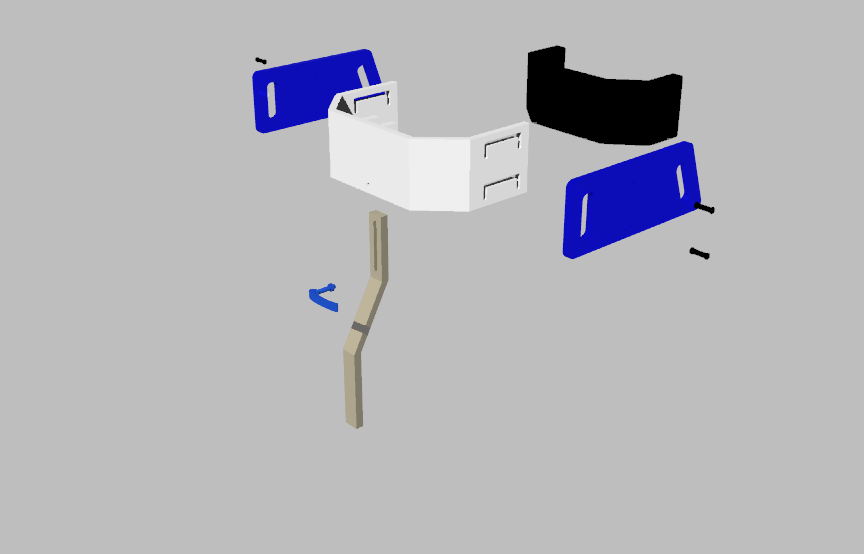
\includegraphics[width=7cm]{images/vistaex2.png}
\caption{Exploded view of the frontrest}
\label{fig:vistaex2}
\end{figure}

\begin{figure}[h]
\centering
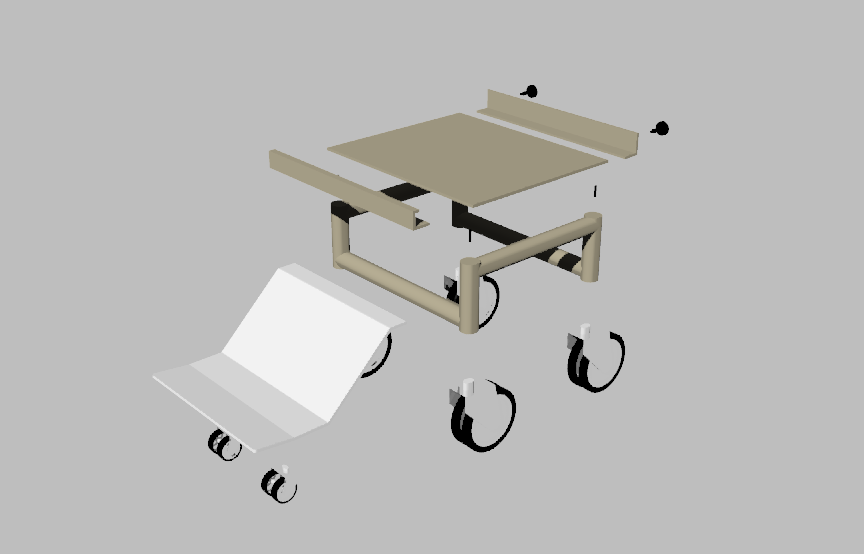
\includegraphics[width=7cm]{images/vistaex3.png}
\caption{Exploded view of the base and footrest}
\label{fig:vistaex3}
\end{figure}

\begin{figure}[h]
\centering
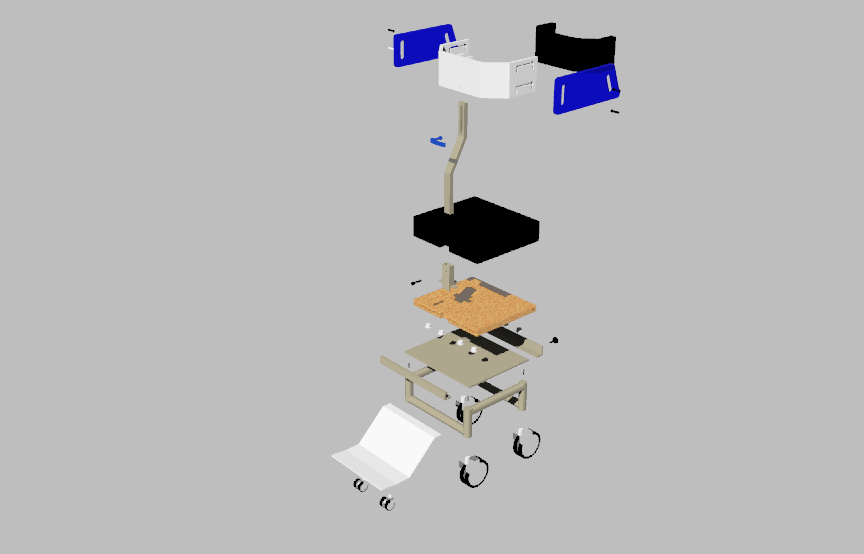
\includegraphics[width=7cm]{images/vistaex4.png}
\caption{Exploded view of  redesigned aisle wheelchair}
\label{fig:vistaex4}
\end{figure}

\begin{figure}[h]
\centering
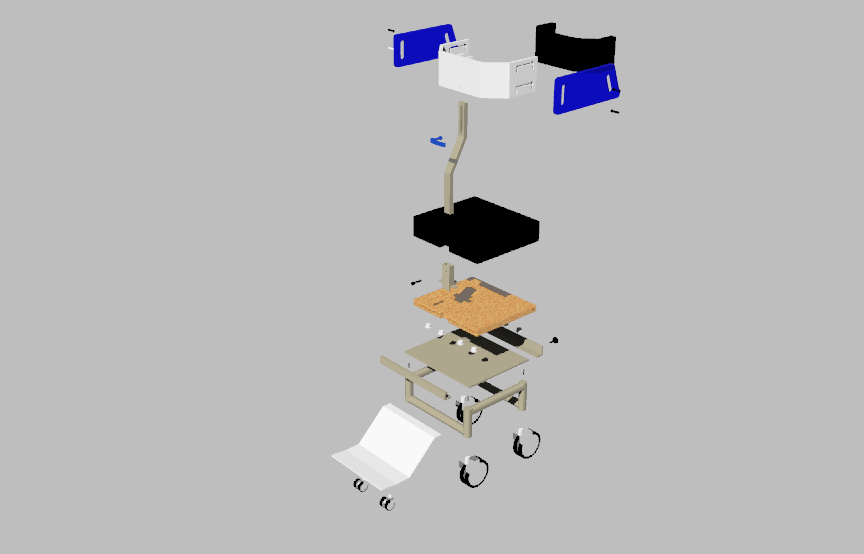
\includegraphics[width=7cm]{images/vistaex4.png}
\caption{Exploded view of  redesigned aisle wheelchair}
\label{fig:vistaex4}
\end{figure}

\begin{figure}[h]
\centering
\includegraphics[width=15cm]{images/almofada.png}
\caption{Frontrest cushion}
\label{fig:frontcushionmodel}
\end{figure}

\begin{figure}[h]
\centering
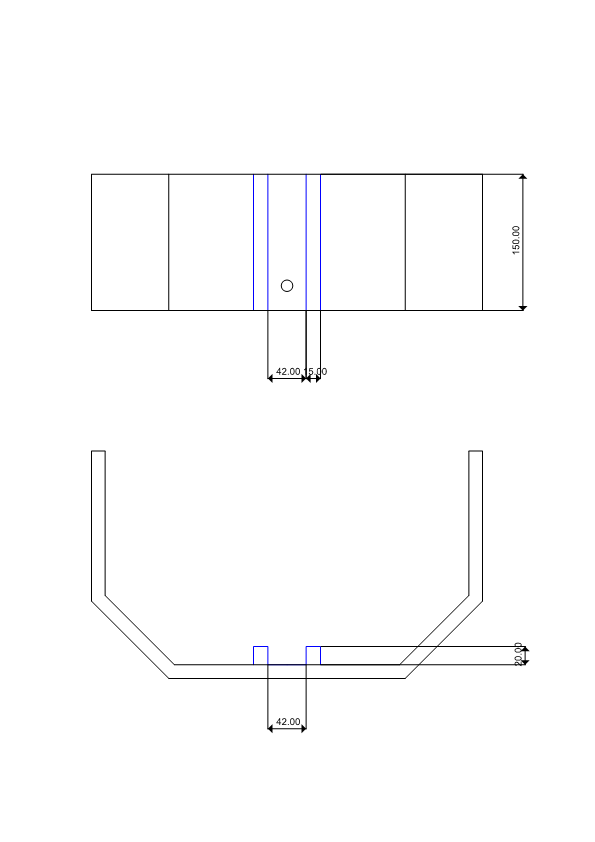
\includegraphics[width=15cm]{images/barra.png}
\caption{Detail of the bar slot on the frontrest}
\label{fig:frontrestslot}
\end{figure}


\begin{figure}[h]
\centering
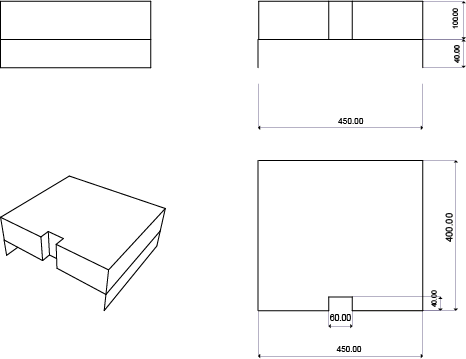
\includegraphics[width=15cm]{images/almofadadebaixo.png}
\caption{Seat cushion}
\label{fig:seatcushion}
\end{figure}

\begin{figure}[h]
\centering
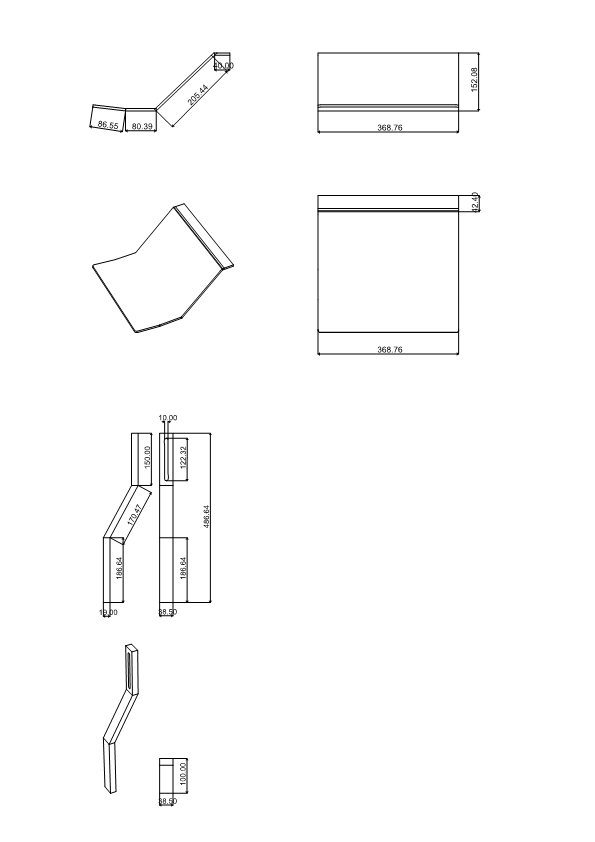
\includegraphics[width=15cm]{images/barraepes.png}
\caption{Front bar and footrest}
\label{fig:frontbarandfootrest}
\end{figure}

\begin{figure}[h]
\centering
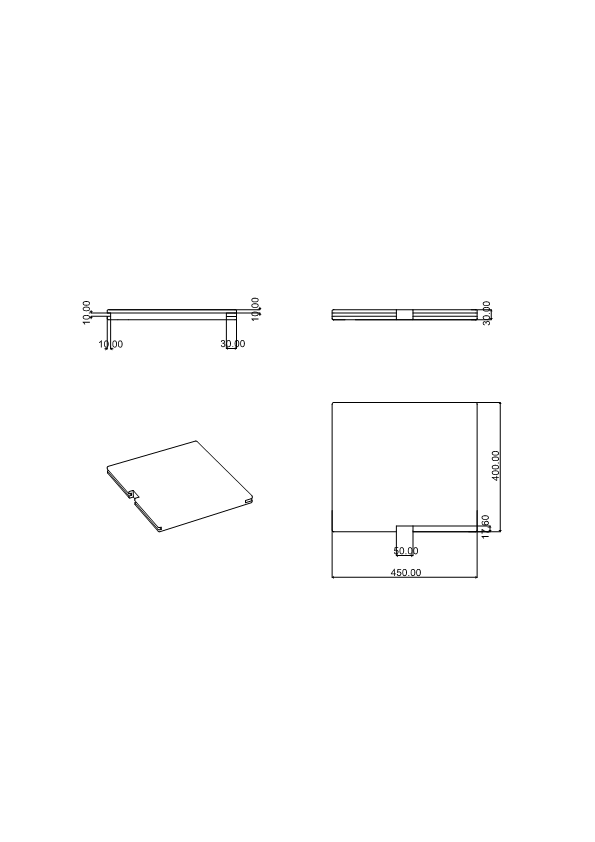
\includegraphics[width=15cm]{images/base.png}
\caption{Base of the wheelhair}
\label{fig:base}
\end{figure}

\begin{figure}[h]
\centering
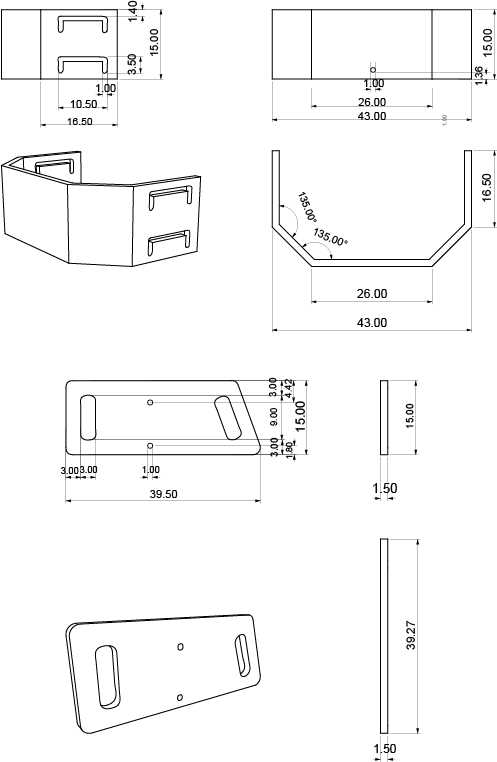
\includegraphics[width=11cm]{images/DesenhoTecnicoApoio.png}
\caption{Front support and handles design}
\label{fig:frontsupport}
\end{figure}

\begin{figure}[h]
\centering
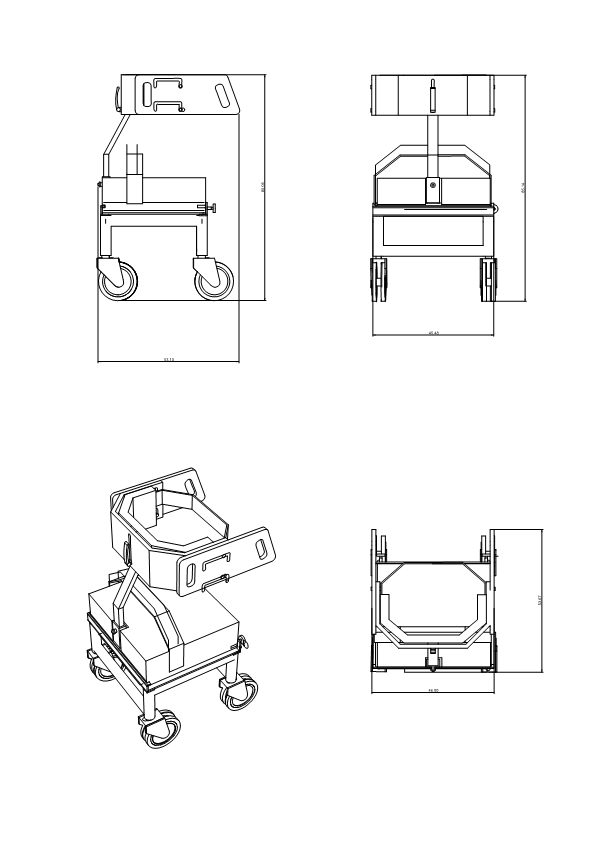
\includegraphics[width=15cm]{images/geral.png}
\caption{Design of the aisle wheelchair}
\label{fig:designwheelchair}
\end{figure}

\begin{figure}[h]
\centering
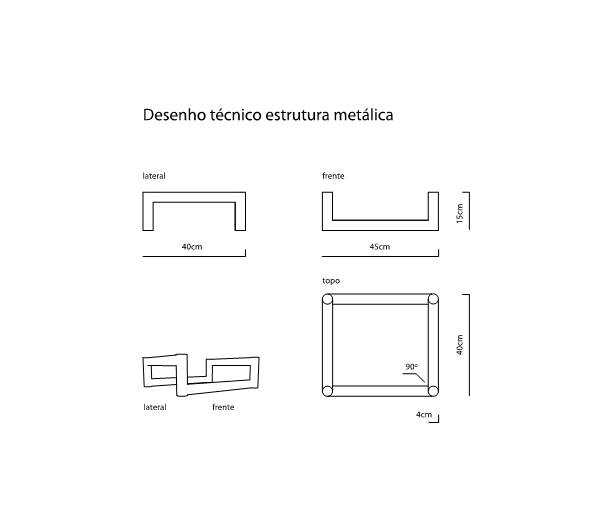
\includegraphics[width=15cm]{images/DesenhoTecnicoEstrutura.png}
\caption{Design of the wheelchair's  structure}
\label{fig:wheelchairstructure4}
\end{figure}

\begin{figure}[h]
\centering
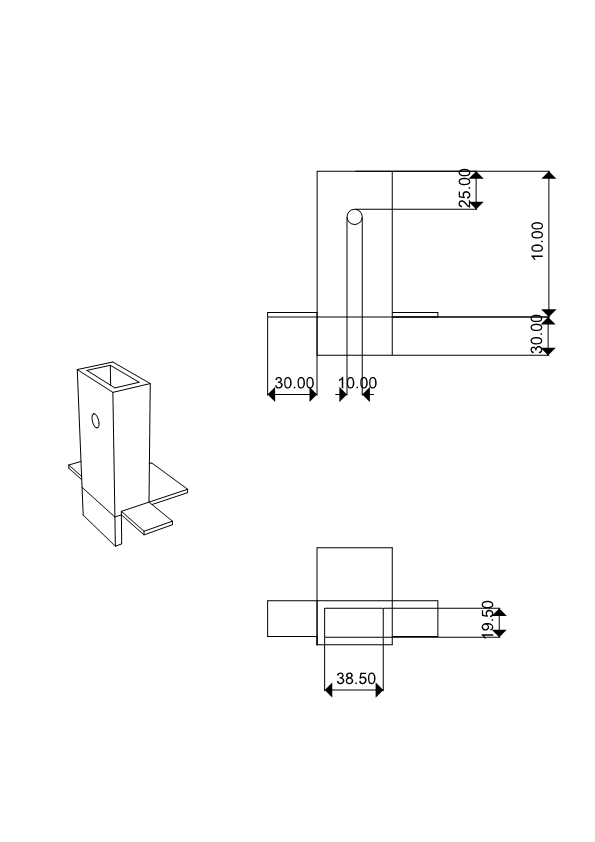
\includegraphics[width=15cm]{images/MastroMedidas2.png}
\caption{Detail of the front support's housing}
\label{fig:housing}
\end{figure}

\begin{figure}[h]
\centering
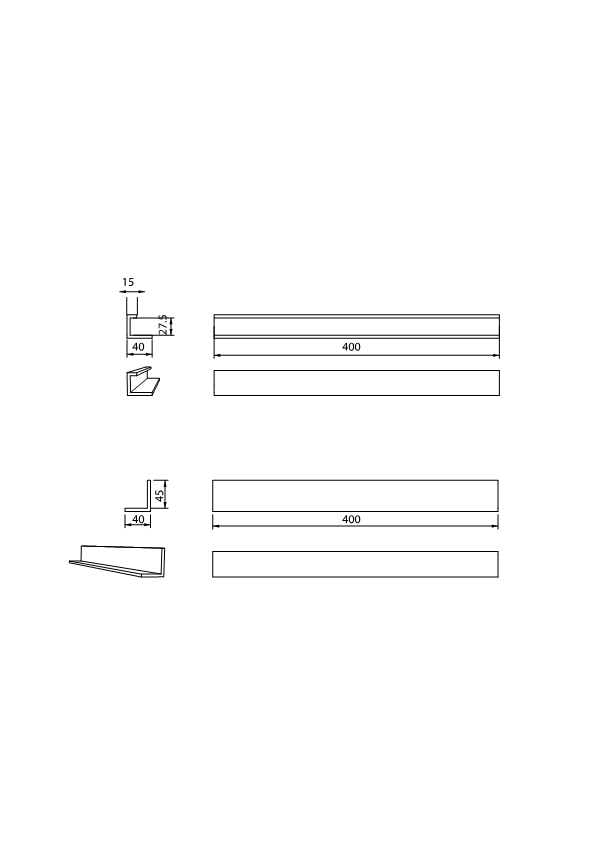
\includegraphics[width=15cm]{images/metaisMedidas.png}
\caption{Details of the aluminum profiles }
\label{fig:aluminumprofiles}
\end{figure}